\chapter{Implementierung}
\label{chap:Implementierung}

%To DO für dieses Kapitel: Abbildung zur Visualisierung der fertigen Verfahren einbinden (Screenshot aus VR), Code schön machen, bei "Strategien zur Fehlervermeidung und Debugging" reflexion ergänzen, wie hilfreich die Ansätze waren (oder weglassen?), Installation & Nutzerdokumentation ergänzen (Verweis auf Anhang mit GitRepo), Bezug zu FF2 herstellen, "Animation der Linien" ersetzen! (Bewegung, Durchlauf o. ä.)

In diesem Kapitel wird die technische Umsetzung der erarbeiten Konzepte beschrieben. Dabei wird zunächst die grundlegende Architektur beschrieben, gefolgt von Grundlagen, die für beide Konzepte gleichermaßen entscheidend sind. Anschließend wird die spezifische Implementierung der beiden Konzepte tiefergehend vorgestellt. Hierbei wird zunächst das Item Scanning beschrieben und anschließend das Cartesain Scanning. Danach werden allgemeine Strategien zur Fehlerbehandlung sowie in der Entwicklung genutzte Debugging-Methoden vorgestellt. Abschließend werden Limitationen aufgezeigt und es wird ein kurzer Ausblick auf mögliche zukünftige Erweiterungen der Implementierung eröffnet. 

\section{Architektur}
Die Implementierung der konzipierten Interaktionsschnittstellen erfolgt innerhalb des Tools PaneoVR. Die Entwicklung dieses Tools erfolgte in der \textit{Game Engine Unity}, dementsprechend werden auch die Implementierungen im Rahmen dieser Arbeit in Unity durchgeführt. 

Die für die Implementierung relevanten Erweiterungen im Rahmen dieser Arbeit wurden in der IngameScene vorgenommen. Nachfolgend sind die zentralen Komponenten dieser Szene aufgeführt, die für die Weiterentwicklung im Rahmen dieser Arbeit relevant waren. 

{\normalfont \bfseries Zentrale Komponenten der IngameScene}

\begin{itemize}
    \item \textit{Interaction Sphere:} Ein GameObject, an dem beim Laden einer neuen Szene alle interaktiven Paneo-Elemente als Child-Objekte angehängt werden.
    \item \textit{Scene Manager:} Enthält u. a. das Script Scene Loader, das für das dynamische Laden der interaktiven Elemente verantwortlich ist. Dieses Script wurde zur Implementierung des Item Scanning erweitert. 
    \item \textit{XRRigMultiplayer:} Wird beim Start der Szene gespawnt und enthält u. a. die Main Camera sowie den UI-Anchor. Dem UI-Anchor sind zentrale UI-Komponenten wie das Ingame-Menü und die Elemente für Nachrichten (Hint-Panel und Verify-Panel) untergeordnet.    
\end{itemize}

{\normalfont \bfseries Erweiterungen der ursprüglichen Szene im Rahmen dieser Arbeit}

Zur Implementierung der Scanning-Methoden wurden mehrere neue GameObjects und zugehörige Skripte in die IngameScene integriert (vgl. \autoref{fig:infofluss}). Diese werden folgend kurz aufgelistet und die wichtigsten Funktionalitäten vorgestellt. 

\begin{figure}[tbhp]
    \centering
    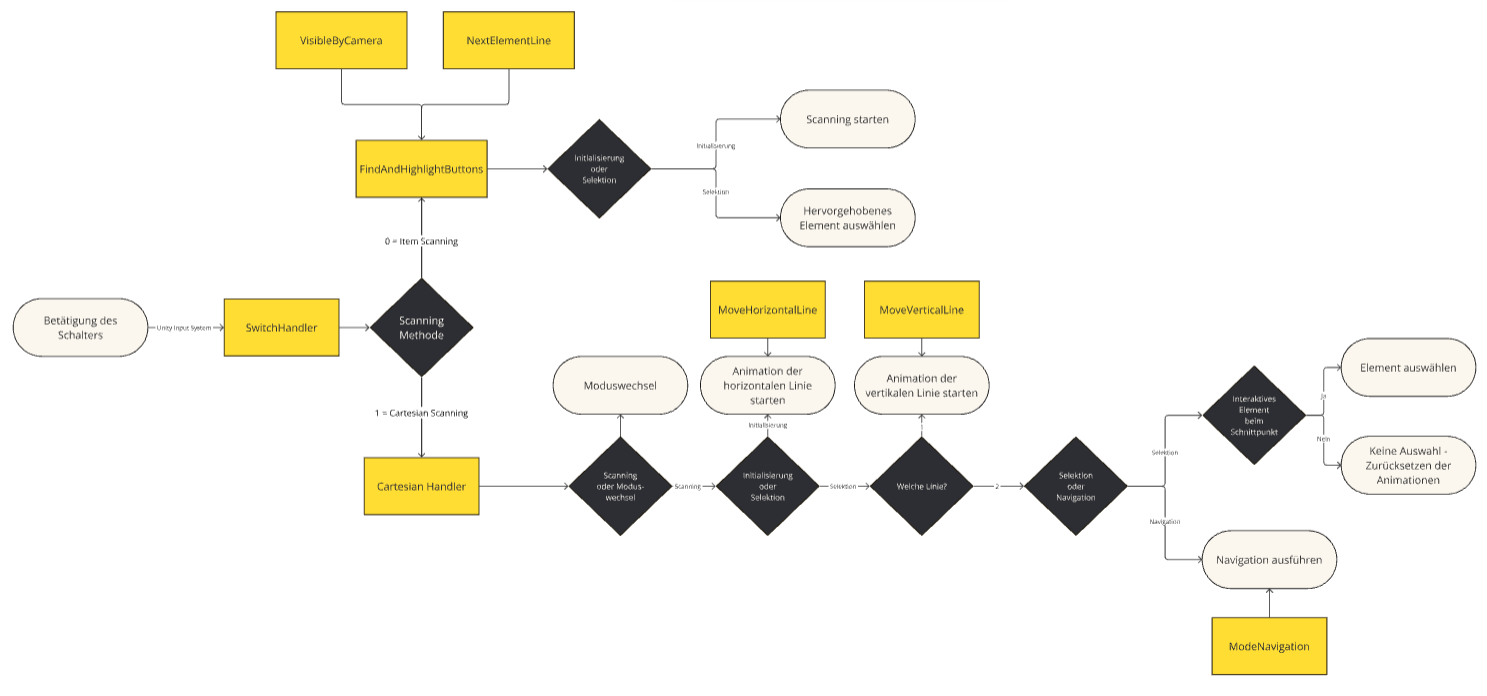
\includegraphics[width=1\textwidth]{images/FlussdiagrammArchitektur.png}
    \caption{Grundlegender Informationsfluss der Softwarearchitektur}
    \label{fig:infofluss}
\end{figure}

\begin{itemize}
    \item \textit{SwitchHandler:}
    Dieses Script verarbeitet die Eingaben des Nutzenden, die über das Unity Input System erfasst werden. Je nach gewählter Scanning-Methode (0 = Item Scanning, 1 = Cartesian Scanning) leitet der SwitchHandler die Eingaben an das entsprechende Script (FindAndHighlightButtons oder Cartesian Handler) weiter. Beim Cartesian Scanning überprüft der SwitchHandler, ob der Schalter länger als zwei Sekunden gehalten wurde, um den Interaktionsmodus zu wechseln.
    \item \textit{FindAndHighlightButtons:}
    Hierbei handelt es sich um das zentrale Script für das Item Scanning. Es führt das schrittweise Hervorheben der interaktiven Elemente in der Szene aus und ermöglicht die Auswahl des aktuell hervorgehobenen Objekts.
    \item \textit{CartesianScanHandler:} 
    Dies ist das zentrale Script für das Cartesian Scanning. Es steuert, zu welchem Zeitpunkt die Animationen der Linien aufgerufen werden, berechnet den Schnittpunkt der Linien, überprüft, ob sich hinter dem Schnittpunkt ein interaktives Element befindet, und führt die Selektion oder einen Moduswechsel aus. 
    \item \textit{VisibleByCamera:}
    Dieses Script ist insbesondere für das Item Scanning relevant und prüft, ob sich ein interaktives Element im Sichtfeld der Kamera befindet.
    \item \textit{NextElementLine:} 
    Dieses Script dient der Visualisierung der Scanning-Reihenfolge im Item Scanning. Durch die hier gesteuerten Animationen wird verdeutlicht, welches Element als nächstes hervorgehoben wird, um die Reihenfolge für Nutzende nachvollziehbar zu gestalten.
    \item \textit{SoundHandler:}
    Dieses Script ist für die Steuerung der Feedback-Audioausgaben bei Interkationen zuständig.
\end{itemize}

Die aufgeführten Skripte kommunizierten größtenteils über direkte Methodenaufrufe miteinander, was eine schnelle und direkte Weiterleitung von Eingaben und Verarbeitungsergebnissen ermöglicht. Um die Übersichtlichkeit und Wartbarkeit des Codes sicherzustellen, wurden die Scanning-Verfahren so gestaltet, dass für jedes ein eigenes Hauptskript mit der wichtigsten Funktionalität erstellt wurde. Dadurch befindet sich die gesamte Logik für jedes Verfahren an einem zentralen Ort. Es ist somit nicht erforderlich, zwischen mehreren Skripten zu wechseln, um spezifische Funktionen zu finden und anzupassen oder zu erweitern. Dennoch wurden einige Funktionen bewusst ausgelagert. Die Prüfung, ob ein Objekt sichtbar im Blickfeld der Kamera ist, wurde in ein separates Skript überführt. So kann diese Prüfung gegebenenfalls unabhängig vom Scanning-Verfahren wiederverwendet werden. Die Methoden zur Animation der Linien im Cartesian Scanning wurden direkt an die animierten Objekte gebunden. Dies erleichtert die Konfiguration der Animationen und fördert eine klare Trennung der Verantwortlichkeiten. Für die Ausführung der Navigation wurden ebenfalls zusätzliche Skripte erstellt. Das Skript \textit{MenuNavigation} realisiert die Rotation des XRRigs beim Item Scanning, während das Skript \textit{ModeNavigation} diese Funktionalität für das Cartesain Scanning übernimmt. Die beiden Funktionalitäten wurden dabei bewusst auf zwei Skripte geteilt, um die Unabhängigkeit der beiden Scanning-Verfahren beizubehalten. 

Der grundlegende Informationsfluss, der zwischen diesen vorgestellten Skripten besteht, wird in \autoref{fig:infofluss} veranschaulicht. Die Eingaben der Nutzenden werden über das Unity Input System erfasst und zunächst im \textit{SwitchHandler} verarbeitet. Abhängig von der gewählten Scanning-Methode wird die Eingabe an den entsprechenden Scanning Handler weitergeleitet. Beim Item Scanning übernimmt das Skript \textit{FindAndHighlightButtons} die schrittweise Hervorhebung der Elemente sowie die Selektion des aktuell hervorgehobenen Elements. Beim Cartesian Scanning steuert der \textit{CartesianScanHandler} die Animation der Linien, die Schnittpunktberechnung und die Auswahl der interaktiven Elemente.

\section {Gemeinsame Komponenten beider Konzepte}

Die Implementierung der beiden Scanning-Methoden basiert u. a. auf gemeinsam genutzten Komponenten, die Funktionalitäten beider Interaktionsschnittstellen unterstützen. Dazu gehören die Eingabeverarbeitung, die Audioausgabe sowie ein zusätzliches Highlight-GameObject, das allen interaktiven Objekten als Kindsobjekt hinzugefügt wird. 

{\normalfont \bfseries Eingabeverarbeitung}

Als Eingabe wurde zunächst eine neue Input Action erstellt, die die Leertaste der Tastatur als Simulation eines Schalters verwendet. Diese Lösung ermöglicht eine einfache Simulation während der Entwicklung und Evaluation, wenn kein Schalter zur Verfügung steht. Für verschiedene Arten von Schaltern kann diese Konfiguration zukünftig leicht erweitert werden.

Für die Verarbeitung von Eingaben wurde das Skript \textit{SwitchHandler} als zentrale Komponente implementiert. Dieses nutzt die Events \textit{started} und \textit{canceled} des Unity Input System, um die Aktionen des Nutzenden zu erkennen und entsprechend zu verarbeiten. Bei der \textit{Started-Action} wird die Methode \textit{OnPressStarted} aufgerufen. In dieser wird der Zeitpunkt des Drückens zwischengespeichert und die Variable \textit{isPressing} wird auf \textit{true} gesetzt. Dies geschieht jedoch nur unter der Voraussetzung, dass das Cartesian Scanning als Scanning-Methode eingestellt ist. In der \textit{Update-Methode} wird daraufhin kontinuierlich überprüft, ob \textit{isPressing} auf \textit{true} steht und ob seit dem Beginn des Drückens bereits zwei Sekunden vergangen sind. Wenn dies der Fall ist, wird ein akustisches Feedback ausgelöst, das dem Nutzenden signalisiert, dass ein Wechsel des Interaktionsmodus bei Loslassen des Schalters durchgeführt wird.
Bei der \textit{Canceled-Action} wird die Methode \textit{OnPressEnded} aufgerufen. Hier wird zunächst geprüft, welche Scanning-Methode eingestellt ist. Ist das Item Scanning aktiv, wird die Eingabe an das \textit{FindAndHighlightButtons}-Skript weitergeleitet. Ist das Cartesian Scanning aktiv, wird zunächst die Dauer des Tastendrucks geprüft. Wurde die Taste länger als zwei Sekunden gedrückt, wird die Methode \textit{changeMode} im \textit{CartesianScanHandler} aufgerufen, um den Interaktionsmodus zu wechseln. Andernfalls wird die Methode \textit{Scanning} aufgerufen, um den Scanning-Vorgang zu starten. Die gewählte Scanning-Methode wird in einer Integer-Variable gespeichert, wobei 0 für das Item Scanning und 1 für das Cartesian Scanning steht. 

{\normalfont \bfseries Audioausgabe}

Die Anwendung bietet Nutzenden akustisches Feedback, das über den \textit{AudioHandler} realisiert wird. Dieser ermöglicht das Erzeugen einer AudioSource zur Laufzeit, die den übergebenen AudioClip abspielt und anschließend automatisch wieder entfernt wird. Diese Implementierung ist ressourcenschonend und verhindert Probleme, die auftreten könnten, wenn eine AudioSource an ein GameObject gebunden ist und dieses während der Laufzeit entfernt wird. Durch diese Lösung wird sichergestellt, dass alle Sounds vollständig abgespielt werden, was insbesondere für Benutzerfeedback von zentraler Bedeutung ist.

{\normalfont \bfseries Highlight Objekt}

Allen interaktiven Objekten wurde ein Highlight-Objekt als Child-Objekt hinzugefügt. Dieses Highlight besteht aus einer einfachen geometrischen Form (Sphere oder Cube), die mit einem transparenten Material versehen ist. Die Geometrie dient dazu, die Darstellung von Outlines zu ermöglichen, da diese nur an sichtbaren Meshes generiert werden können. Das Highlight-Objekt enthält zudem einen Mesh Renderer (initial deaktiviert), einen Collider und eine Outline, die mithilfe des kostenlosen Plugins Quick Outline \citep{chris_nolet_quick_2022} aus dem \textit{Unity Asset Store} realisiert wurde.
Das Highlight-Objekt wird von beiden Scanning-Methoden unterschiedlich genutzt. Beim Item Scanning wird die Outline durch Aktivieren des Mesh Renderers sichtbar gemacht, um zu visualisieren, dass dieses Objekt ausgewählt werden kann. Zusätzlich wird der Collider verwendet, um zu prüfen, ob das Objekt im Sichtfeld der Kamera liegt. Beim Cartesian Scanning wird der Collider ebenfalls verwendet. In diesem Zusammenhang jedoch um zu prüfen, ob hinter dem Schnittpunkt der Linien ein interaktives Objekt liegt. Auf die genaue Funktionsweise des Highlight-Objekts in den spezifischen Kontexten wird folgend in der Vorstellung der beiden Konzepte genauer eingegangen. 

\section{Scanning-Verfahren}

\subsection{Konzept 1 - Item Scanning }

Das Item Scanning basiert auf einer Liste, die alle interaktiven Elemente einer Szene enthält. Diese interaktiven Elemente (Interactables) werden beim Laden einer Szene durch das Skript \textit{SceneLoader} erzeugt und automatisch der Liste im Skript \textit{FindAndHighlightButtons} hinzugefügt. Zusätzlich werden zwei UI-Buttons hinzugefügt, die immer als HUD sichtbar sind. Dabei handelt es sich um einen Button zum Öffnen des Menüs und einen Button zum Öffnen des Navigationsmenüs. Sobald der \textit{SwitchHandler} eine Eingabe registriert, prüft er, ob das Scanning bereits aktiv ist oder initialisiert werden muss. Diese Information wird über einen Methodenaufruf an das Skript \textit{FindAndHighlightButtons} übergeben. Ist das Scanning noch nicht aktiv, wird die Methode \textit{StartItemScanning} aufgerufen, andernfalls die Methode \textit{SwitchSelection}. Diese beiden Methoden stellen die zentrale Funktionalität der Scanning-Methode dar. Im Folgenden werden diese und weitere relevante Aspekte näher beschrieben.

\textbf{Start und Verlauf des Scannings}

Die Methode \textit{StartItemScanning} startet eine Coroutine namens ItemScanning, in der der eigentliche Scan-Vorgang abläuft. Diese Coroutine iteriert über die Liste der interaktiven Elemente und hebt sie nacheinander hervor. Der Ablauf ist im folgenden Pseudocode \autoref{lst:codeItem} vereinfacht dargestellt.

\begin{lstlisting} [language={[Sharp]C}, caption=Vereinfachter Pseudocode des Item Scannings, label={lst:codeItem}]

IEnumerator ItemScanning()
{
    while (isScanActive)
    {
        foreach (GameObject button in allButtons)
        {
            // Versuche, das Highlight-Objekt zu finden
            GameObject highlight = button.transform.Find("Highlight").gameObject;
            
            if (highlight != null)
            {
                // Pruefe, ob das Highlight-Objekt sichtbar ist
                if (visibleByCamCheck.IsVisibleByCam(cam, highlight.GetComponent<Collider>()))
                {
                    // Aktiviere das Highlight-Objekt
                    highlight.GetComponent<MeshRenderer>().enabled = true;
                    highlightedObject = button;

                    // Starte die Animation zum naechsten Objekt
                    GameObject nextObject = GetNextHighlightableObject();
                    scriptNextElement.DrawLineBetweenElements(highlightedObject, nextObject);

                    // Warte fuer die Scan-Rate
                    yield return new WaitForSeconds(ScanRate);

                    // Deaktiviere das Highlight-Objekt, falls es noch existiert
                    if (highlight != null)
                    {
                        highlight.GetComponent<MeshRenderer>().enabled = false;
                    }
                }
            }
        }
    }
}

\end{lstlisting}

Die Iteration läuft, solange das Scanning aktiv ist. Für das aktuelle Objekt wird zunächst geprüft, ob es ein Highlight-GameObject als Kind-Objekt enthält. Diese Prüfung stellt sicher, dass wirklich nur Objekte in den Scan-Vorgang einbezogen werden, die auch visuell hervorgehoben werden sollen. Ist ein Highlight-Objekt vorhanden, wird über den Collider des Objekts ermittelt, ob es sich aktuell im Sichtfeld der Kamera befindet. Dies geschieht über das Skript \textit{VisibleByCamera}.
Ist diese Prüfung positiv, wird das Highlight durch Einschalten des Mesh Renderers aktiviert. Gleichzeitig wird das hervorgehobene Objekt in einer entsprechenden Variablen gespeichert, um bei der Selektion darauf zugreifen zu können. Anschließend wird das nächste hervorzuhebende Objekt bestimmt und eine Animation gestartet, die eine Linie zwischen dem aktuellen und dem nächsten Objekt visualisiert. Diese Animation wird weiter unten ausführlicher behandelt. Nach Ablauf der Wartezeit, die durch die Scan Rate bestimmt wird, wird der Mesh Renderer des Highlight-Objektes wieder deaktiviert, sofern das Objekt noch existiert. Dies ist notwendig, da das Objekt unter Umständen während der Wartezeit gelöscht werden kann. Würde an dieser Stelle keine erneute Überprüfung erfolgen, käme es zu einer NullPointerException.


\textbf{Auswahl eines interaktiven Elements}

Die Auswahl eines hervorgehobenen Elements erfolgt über die Methode SwitchSelection. Hier wird geprüft, ob ein Objekt aktuell hervorgehoben ist. Ist dies der Fall, wird die Button-Komponente des Objekts gesucht und deren OnClick-Event ausgelöst. Der Ablauf ist im folgenden Pseudocode \autoref{lst:selectItem} veranschaulicht.

\begin{lstlisting} [language={[Sharp]C}, caption=Vereinfachter Pseudocode der Selektion des Item Scanning, label={lst:selectItem}]

public void SwitchSelection()
{
    if (highlightedObject != null)
    {
        // Suche nach der Button-Komponente
        GameObject buttonTrigger = highlightedObject.transform.Find("Btn_Trigger").gameObject;
        Button buttonToClick = buttonTrigger.GetComponent<Button>();

        // Loese das OnClick-Event aus
        if (buttonToClick != null)
        {
            ExecuteEvents.Execute(
                buttonToClick.gameObject,
                new BaseEventData(EventSystem.current),
                ExecuteEvents.submitHandler
            );
        }
    }
}
    
\end{lstlisting}

Die gleiche Logik wird für die Navigation verwendet. Wenn ein Pfeilbutton im Navigationsmenü ausgewählt wird, wird das OnClick-Event des Buttons ausgelöst, welches wiederum die Methode turnLeft bzw. turnRight im Skript MenuNavigation aufruft. Diese Methoden drehen das XRRig um 40° (rechts) bzw. -40° (links).

\textbf{Animation zwischen dem aktuellen und folgenden Element}

Um die Reihenfolge zu verdeutlichen, in der die interaktiven Objekte hervorgehoben werden, wird eine Linie zwischen dem aktuellen und dem nächsten Element gezogen. Dazu wurde der \textit{IngameScene} das GameObject \textit{NextElementLine} hinzugefügt. Dieses enthält einen Line Renderer zur Darstellung der Linie sowie das Skript \textit{NextElementLine}, das die Steuerung der Animation übernimmt.
Die Animation wird als Coroutine umgesetzt. Der Startpunkt der Linie ist die Position des aktuell hervorgehobenen Elements, der Endpunkt die Position des nächsten Elements. Die Sichtbarkeit der Linie wird über die AlphaKeys des Line Renderers gesteuert, die von 0 auf 1 gesetzt werden. Dadurch wird die Linie schrittweise sichtbar. Die Animationsdauer entspricht der Scan Rate. Damit die Linie die Position dynamischer UI-Elemente korrekt darstellt, werden Start- und Endpunkte in der Update-Methode jeden Frame aktualisiert.

\textbf{Herausforderungen}

Die Herausforderungen bei der Implementierung des Item Scanning lagen insbesondere in der Unterscheidung der verschiedenen Ebenen. Wird z. B.  ein Menü oder ein Dialogfeld geöffnet, so muss das Scanning auf diese Teilauswahl von Items beschränkt werden. Die Lösung dieses Problems wird im Folgenden exemplarisch an einem Dialog-Interactable beschrieben. 
Wird das Dialog-Objekt innerhalb des Item Scanning ausgewählt, wird das OnClick-Ereignis ausgelöst. Dadurch wird die Methode DialogScan aufgerufen. Dieser Methode werden beim Aufruf die Buttons der Antwortoptionen übergeben. Aus diesen Optionen wird ein Array erstellt, das dann mit der oben beschriebenen Logik durchlaufen werden kann. Die Auswahloptionen müssen also dynamisch angepasst werden, je nachdem welches Objekt aktiv ist bzw. sich auf der vordersten Ebene befindet. Dies erfordert besondere Aufmerksamkeit bei der Implementierung, da verschiedene Fälle berücksichtigt werden müssen. Für jedes Objekt, das eine weitere Ebene öffnet, muss geprüft werden, wie sich die Auswahl der Scan-Optionen dadurch ändert. 
Eine weitere Herausforderung bei der Implementierung des Item Scanning bestand darin, das Scanning-Set dynamisch auf die Elemente zu beschränken, die sich im aktuellen Sichtfeld des Nutzenden befinden. Die Herausforderung bestand darin, eine Lösung zu finden, die die Performance der Anwendung nicht wesentlich beeinträchtigt. Dies ist insbesondere bei größeren Kopfbewegungen relevant, bei denen sich das Sichtfeld abrupt und deutlich ändert und das Scanning-Set entsprechend schnell und ressourcenschonend angepasst werden muss.

\subsection{Konzept 2 - Cartesian Scanning}

Um das Cartesian Scanning zu implementieren, wurden zwei neue GameObjects erstellt und der Kamera im XRRig untergeordnet. Diese GameObjects enthalten jeweils ein Canvas, das annähernd auf die Größe des Sichtfeldes skaliert ist. Auf diesem Canvas befindet sich wiederum ein GameObject mit einer Rect Transform-Komponente, einem Line Renderer zur Darstellung der Linien sowie dem Skript \textit{MoveHorizontalLine} bzw. \textit{MoveVerticalLine}. Die GameObjects sind zu Beginn der Anwendung deaktiviert und werden erst während des Scan-Vorgangs aktiviert.
Die horizontale Linie bewegt sich von oben nach unten vor dem Nutzenden, während die vertikale Linie sich von links nach rechts bewegt. Die Bewegung der Linien wird über die genannten Skripte gesteuert. Der Aufbau dieser Skripte wird im Folgenden näher beschrieben. 

\textbf{Animation der Linien}

Die Methode \textit{StartAnimation} startet die Coroutine \textit{MoveLine}, in der die Bewegung der Linie gesteuert wird. Hier wird zunächst die Start- und Endposition der Linie definiert. Bei der horizontalen Linie sind dies der obere und der untere Rand des Canvas. Bei der vertikalen Linie entspricht dies dem linken und rechten Rand des Canvas. Nachfolgend ist in \autoref{lst:moveLine} ein Ausschnitt aus dieser Coroutine zur Veranschaulichung der Bewegung dargestellt. 

\begin{lstlisting} [language={[Sharp]C}, caption=Ausschnitt aus der Methode zur Animation der Linien im Cartesian Scanning, label={lst:moveLine}]

while (currentTime <= scanRate)
{
    currentTime += Time.deltaTime;
    normalizedValue = currentTime / scanRate;
    rectTransform.anchoredPosition = Vector3.Lerp(startPosition, endPosition, normalizedValue);
    yield return null;
}
\end{lstlisting}

Sobald die Linie ihre Endposition erreicht hat, wird über eine Zählervariable geprüft, ob die Animation bereits dreimal hintereinander ausgeführt wurde. Ist die Linie noch nicht dreimal durchgelaufen, wird die Animation zurückgesetzt und erneut gestartet. Erst nach dem dritten Durchlauf wird die Reset-Methode im CartesianScanHandler aufgerufen, wo der gesamte Fortschritt des Scanning zurückgesetzt wird. Dieses wiederholte Durchlaufen wurde zur Fehlerkorrektur implementiert. Wird die gewünschte Position der Linie beim ersten Durchlauf verfehlt, kann einfach abgewartet werden, bis die Linie wieder die gewünschte Position erreicht hat. Durch den Abbruch nach drei Durchläufen werden zudem vermeidbare Fehlauswahlen vermieden.

Eine weitere wesentliche Methode innerhalb des Skripts ist \textit{StopAnimation}. Diese bewirkt, dass die aktuell laufende Coroutine gestoppt wird, sodass die Linie in ihrer aktuellen Position verbleibt. Die Methode wird aufgerufen, sobald Nutzende die Position der Linie im Zuge des Scanning setzen möchten.

\textbf{Steuerung des Scanning-Prozesses}

Die eigentliche Steuerung des Cartesian Scanning erfolgt im Skript \textit{CartesianScanHandler}. Wird im \textit{SwitchHandler} eine Eingabe registriert, wird die Methode Scanning im \textit{CartesianScanHandler} aufgerufen. Diese prüft, in welchem Stadium sich der Scanning-Prozess befindet, und ruft entsprechend die nächste erforderliche Methode auf (vgl. \autoref{lst:scanningCartesian}). 

\begin{lstlisting} [language={[Sharp]C}, caption=Methode Scanning im CartesianScanHandler, label={lst:scanningCartesian}]

public void Scanning()
{
    if (!firstStarted)
    {
        ScanningFirstLine();
    }
    else
    {
        if (!secondStarted)
        {
            StopFirstLine();
        }
        else
        {
            Selection();
        }
    }
}
    
\end{lstlisting}

Die Methode \textit{ScanningFirstLine} aktiviert das GameObject der horizontalen Linie und ruft die Methode \textit{StartAnimation} im Skript \textit{MoveHorizontalLine} auf. In der Methode \textit{StopFirstLine} wird diese durch den Methodenaufruf \textit{StopAnimation} gestoppt, das GameObject der vertikalen Linie aktiviert und die Animation gestartet. In der Methode \textit{Selection} wird anschließend die Animation der zweiten Linie gestoppt, die beiden GameObjects wieder deaktiviert, die Animationen zurückgesetzt und die Variablen \textit{firstStarted} und \textit{secondStarted} wieder auf false gesetzt. Um die Selektion durchzuführen, wird die Methode \textit{FindIntersection} aufgerufen. Hier wird der Schnittpunkt der Linien berechnet. Dies wird im Folgenden anhand von Pseudocode veranschaulicht. 

\begin{lstlisting} [language={[Sharp]C}, caption=Pseudocode zur Veranschaulichung der Methode FindIntersection im CartesianScanHandler, label={lst:scanningCartesian}]

    public void FindIntersection()
    {
        // Positionen der Linien im Canvas Space
        Vector2 horizontalLinePosition = horizontalLine.anchoredPosition;
        Vector2 verticalLinePosition = verticalLine.anchoredPosition;
        
        // Berechnung Schnittpunkts Canvas Space
        Vector2 intersectionInCanvasSpace = new Vector2(verticalLinePosition.x, horizontalLinePosition.y );
        
        // Umwandlung in Weltkoordinaten
        Vector3 intersectionWorldPosition = horizontalLine.transform.parent.TransformPoint(intersectionInCanvasSpace);

        // Selektionsmodus ist aktiv
        if (!navModeActive)
	    {
            CheckForInteractiveElement(intersectionWorldPosition);
        }
        // Navigationsmodus ist aktiviert
        else
        {
            modeNav.turn(intersectionWorldPosition);
        }
    }

\end{lstlisting}

Je nachdem, welcher Modus aktiv ist, wird anschließend unterschiedlich verfahren. Ist der Selektionsmodus aktiviert, wird mit Hilfe der Methode \textit{CheckForInteractiveElement} überprüft, ob sich hinter dem Schnittpunkt der Linien ein interaktives Objekt befindet. Dazu wird mittels eines SphereCasts ein Ray von der Kameraposition durch den berechneten Schnittpunkt erzeugt. An dieser Stelle wurde ein SphereCast anstelle eines einfachen Rays gewählt, um einen Toleranzbereich in Form eines Radius einführen zu können. Dadurch wird ein Objekt auch dann ausgewählt, wenn der Schnittpunkt das Objekt knapp verfehlt. Es wird geprüft, ob dieser Ray den Collider eines Highlight-Objektes getroffen hat. Ist dies der Fall, wird wie beim Item Scanning das OnClick-Event der Button-Komponente des entsprechenden Objekts ausgelöst. Trifft der Ray auf mehrere Objekte, z. B.  wenn zwei Ebenen mit interaktiven Elementen übereinander liegen, wird stets das Objekt ausgewählt, auf das der Ray zuerst trifft. Das heißt, es wird das Element ausgewählt, das näher an der Kamera positioniert ist. Dadurch wird sichergestellt, dass UI-Elemente wie das Ingame-Menü oder das Hint-Panel bevorzugt ausgewählt werden und keine unbeabsichtigten Selektionen bei Verdeckungen auftreten. Wurde kein Objekt getroffen, wird lediglich ein Audio-Feedback ausgelöst. 

Im Navigationsmodus hingegen wird die Methode \textit{turn} im Skript ModeNavigation aufgerufen. Hier wird die y-Koordinate des Schnittpunkts genutzt, um die Rotation des XRRigs entsprechend anzupassen.

\textbf{Wechsel zwischen Selektions- und Navigationsmodus}

Wird im \textit{SwitchHandler} registriert, dass der Schalter länger als 2 Sekunden gehalten wurde, wird die Methode \textit{changeMode} im \textit{CartesainScanHandler} aufgerufen. In dieser Methode wird die boolesche Variable \textit{navModeActive} entsprechend geändert. War diese zuvor auf true, so wird sie nun auf false gesetzt und umgekehrt. Außerdem wird die Farbe der Linie Renderer angepasst. Ist der Navigationsmodus aktiv, werden die Linien blau dargestellt, ist der Selektionsmodus aktiv, werden die Linien pink dargestellt. Dies dient dazu, den Nutzenden eine visuelle Rückmeldung darüber zu geben, welcher Modus gerade aktiv ist. Bei der Auswahl der Farben wurde darauf geachtet, dass diese einen relativ hohen Kontrast aufweisen, damit der Unterschied möglichst auch für Menschen mit Farbschwäche wahrnehmbar ist. 

\textbf{Herausforderungen}

Die Implementierung des Cartesian Scanning war insgesamt aufwendiger als die Implementierung des Item Scanning. Es werden mehr Objekte und Skripte benötigt, um das Scanning zu realisieren. Ist das Grundprinzip jedoch einmal implementiert, ist es vergleichsweise stabil. Ein Vorteil dieses Scanning-Verfahren liegt insbesondere darin, dass Objekte auf unterschiedlichen Ebenen nicht separat betrachtet werden müssen. Dadurch kann die Implementierung insgesamt einfacher um neue Interaktionselemente erweitert werden. 
Eine Herausforderung bei der Implementierung war die Berechnung des korrekten Schnittpunktes sowie die Festlegung eines geeigneten Radius für den SphereCast. Bei der Berechnung des Schnittpunktes musste berücksichtigt werden, dass sich die Linien auf einem Canvas befinden und somit ihre Position in Abhängigkeit von diesem bestimmt wird. Um die tatsächliche Position in Weltkoordinaten zu erhalten, muss zunächst eine Umrechnung erfolgen. Die Festlegung des Radius des SphereCasts stellte eine Herausforderung dar, da hier ein Kompromiss gefunden werden musste. Der Radius musste groß genug sein, um kleine Verfehlungen zu tolerieren, aber klein genug, um bei dicht beieinanderliegenden Objekten eine korrekte Auswahl zu ermöglichen. Es galt also, verschiedene Werte auszuprobieren und zu prüfen, ob sich das gewünschte Ergebnis einstellt. 

\section{Strategien zur Fehlervermeidung und Debugging}

Um Fehlermeldungen vorzubeugen und die Anwendung robuster zu gestalten, wurde an vielen Stellen im Code mit try and catch Abfragen gearbeitet. Insbesondere NullPointerExceptions werden so abgefangen. Dies wird z. B. beim Item Scanning verwendet. Wenn bspw. ein Objekt kein Highlight-Objekt hat oder das Objekt zur Laufzeit der Coroutine gelöscht wird, wird dies abgefangen und das Objekt kann problemlos übersprungen werden. Des Weiteren wurde viel mit boolschen Variablen gearbeitet, um die Abläufe besser verfolgen und steuern zu können. So wird z. B. verhindert, dass zwei Item Scanning Prozesse gleichzeitig gestartet werden. Beim Cartesian Scanning geben die Funktionen bei der Selektion, also CheckForInteractiveElement und modeNav.turn, boolsche Werte zurück, die eine Rückmeldung darüber liefern, ob die Ausführung erfolgreich war. So können die verschiedenen Ausgänge mit unterschiedlichem Audio-Feedback kommuniziert werden. 

Für das Debugging wurde insbesondere die Debug-Klasse von Unity verwendet. An mehreren Stellen wurden Debug.Logs eingefügt, um den Ablauf besser nachvollziehen zu können und schneller zu erkennen, an welcher Stelle im Code Fehler auftreten. Für das Cartesian Scanning wurden zusätzlich einzelne Schritte visuell veranschaulicht. So wurde bspw. während der Entwicklung ein Testobjekt in Form eines einfachen Würfels an die Position des berechneten Schnittpunktes gelegt, um leichter überprüfen zu können, ob dieser korrekt berechnet wird. Ebenso wurde der SphereCast mittels Debug.DrawRay visualisiert, um in der Scene View überprüfen zu können, ob dieser korrekt gezeichnet wird.


\section{Limitationen und mögliche Erweiterungen}

Da die vorliegende Arbeit eine prototypische Implementierung umfasst, bestehen noch mehrere Limitationen, die zukünftige Weiterentwicklungen erforderlich machen.
Im Rahmen der Implementierung wurde die Leertaste eines Laptops als Ersatz für einen physischen Schalter verwendet, um die Interaktion zu simulieren. Für den praktischen Einsatz mit einem physischen Schalter müssten Anpassungen vorgenommen werden, um sicherzustellen, dass der Input eines Schalters korrekt erkannt und verarbeitet wird. 

Eine zentrale Einschränkung beim Item Scanning liegt in der fehlenden Konfigurierbarkeit der Reihenfolge, in der interaktive Objekte hervorgehoben werden. Gegenwärtig basiert die Reihenfolge auf der Reihenfolge, in der die Objekte beim Laden der Szene erzeugt werden. Dies kann dazu führen, dass in der Szene räumlich nahe beieinander liegende Objekte nicht nacheinander hervorgehoben werden, was von Nutzenden als nicht erwartungskonform wahrgenommen werden könnte. Um dieses Problem zu beheben, könnte ein Parameter „Position im Scanning“ in die Prefabs der interaktiven Objekte integriert werden. Durch eine Sortierung der Liste der interaktiven Objekte anhand dieses Parameters könnte die Reihenfolge an die räumliche Anordnung angepasst werden. Dieser Parameter könnte anschließend entweder in Webeditor von PaneoVR oder im Editor-Modus eingestellt werden. 

Eine weitere Limitation betrifft die Konfigurierbarkeit der Scan Rate und des Scanning-Verfahren. Diese Einstellungen können derzeit nur über den Unity-Editor angepasst werden, sodass die Nutzenden keine Möglichkeit haben, diese direkt innerhalb der Anwendung zu ändern. Diese Einschränkung wurde bewusst in Kauf genommen, um die Durchführung der Evaluation zu vereinfachen und vergleichbare Ergebnisse zu gewährleisten. Dies wird in \autoref{chap:Evaluation} ausführlicher erläutert. 
Für den späteren produktiven Einsatz der Scanning-Verfahren wäre jedoch eine entsprechende Anpassungsoption notwendig, um die individuellen Präferenzen und Bedürfnisse der Nutzenden berücksichtigen zu können.

Beim Catesian Scanning stellt die Platzierung der Linien auf einem an das Sichtfeld der Nutzenden angepassten Canvas eine mögliche Einschränkung dar. Für einige Nutzende könnte dies möglicherweise nicht optimal sein. Zukünftige Entwicklungen könnten hier Anpassungsoptionen für den Scan-Bereich vorsehen, um die Benutzerfreundlichkeit zu erhöhen. Eine weitere Einschränkung liegt in der planaren Darstellung der Linien auf einer Ebene. Es wäre sinnvoll zu untersuchen, ob eine sphärische Darstellung, die sich an der Sphäre des 360-Grad-Videos orientiert, die Interaktion noch natürlicher gestalten und die Präzision erhöhen könnte.

Außerdem könnte getestet werden, ob ein multimodales Feedback das Cartesian Scanning noch unterstützen könnte. Beim Item Scanning wurde bspw. ein Audiosignal hinzugefügt, das jedes Mal ertönt, wenn ein neues Objekt hervorgehoben wird. Ein ähnliches Prinzip könnte beim Cartesian Scanning eingeführt werden. Hier könnte bspw. ein Audiosignal ertönen, wenn eine Linie während der Aniamtion mit einem interaktiven Objekt kollidiert. 

\section{Installation, Nutzerdokumentation}

Der Abschnitt fehlt noch - whoops 

Unbedingt zur Implementierung gehört dann am Ende auch eine Beschreibung, wie man die Implementierung zu nutzen hat. Dazu gehört die Beschreibung, wie man die Implementierung bezieht und installiert, genauso wie eine kurze Beschreibung der Bedienung. Falls letztere zu umfangreich werden würde, aber notwendig ist, kann diese auch im Anhang aufgeführt und mit einem Verweis gearbeitet werden.
